% arara: lualatex: { synctex: yes }
% arara: lualatex: { synctex: yes } if found('log', 'undefined references') || found('log', 'Rerun to get cross-references right')
\documentclass{scrartcl}
\usepackage[pretty,polish]{mystd}
\title{Teoria obliczeń i złożoności obliczeniowej}
\author{Michał Dobranowski}
\date{semestr zimowy 2024 \\ v0.2}
\publishers{\github}

\newcommand{\blank}{\square}
\newcommand{\REclass}{\textsf{RE}}
\newcommand{\Rclass}{\textsf{R}}
\newcommand{\coREclass}{\textsf{co-RE}}
\newcommand{\TIME}{\textsf{TIME}}
\newcommand{\SPACE}{\textsf{SPACE}}
\newcommand{\Pclass}{\textsf{P}}
\newcommand{\PSPACEclass}{\textsf{PSPACE}}
\newcommand{\EXPclass}{\textsf{EXP}}
\newcommand{\EXPSPACEclass}{\textsf{EXPSPACE}}
\newcommand{\NPclass}{\textsf{NP}}
\newcommand{\encode}[1]{\left\langle #1 \right\rangle}

\usepackage{algpseudocodex}

\begin{document}
    \maketitle
    \tableofcontents
    \newpage

    \section{Maszyna Turinga i enumerator}

\begin{definition}
    Maszyna Turinga to krotka
    \[ M = (Q, \Sigma, \Gamma, \delta, q_0, q_Y, q_N, \blank),\]
    gdzie
    \begin{itemize}[noitemsep]
        \item $Q$ to skończony zbiór stanów,
        \item $\Sigma$ to skończony alfabet wejściowy,
        \item $\Gamma$ to skończony alfabet taśmy taki, że $\Sigma \subset \Gamma$ oraz $\blank \in \Gamma \setminus \Sigma$,
        \item $\delta : Q \times \Gamma \to Q \times \Gamma \times \{\hookleftarrow , \hookrightarrow\}$ to funkcja przejścia,
        \item $q_0 \in Q$ to stan początkowy,
        \item $q_Y \in Q$ to stan akceptujący,
        \item $q_N \in Q$ to stan odrzucający.
    \end{itemize}
    Formalizację działania maszyny Turinga pozostawiamy jako ćwiczenie dla Czytelnika oraz odsyłamy do podręczników \cite{GareyJohnson, Sipser}.
\end{definition}

Maszyna Turinga (będziemy ją zwali po prostu \enquote{maszyną}) rozwiązuje pewien problem decyzyjny, czyli dla danego słowa $x$ z języka $\Sigma^*$ stwierdza, czy $x$ należy do języka $L \subseteq \Sigma^*$. Dlatego też często będziemy używać pewnych określeń języka również dla odpowiadającego mu problemu decyzyjnego.

Maszyna $M$ \vocab{akceptuje} język $L$, jeśli dla każdego $x \in \Sigma^*$, $M$ akceptuje $x$ wtedy i tylko wtedy, gdy $x \in L$. Przez $L(M)$ oznaczamy język akceptowany przez maszynę $M$.

Maszyna $M$ \vocab{rozstrzyga} o języku $L$, jeżeli go akceptuje i kończy działania dla każdego $x \in \Sigma^*$. Jeśli taka maszyna istnieje, to mówimy, że język $L$ jest \vocab{rozstrzygalny}. Również problem decyzyjny odpowiadający językowi $L$ nazywamy rozstrzygalnym.

\subsection{Klasy $\REclass$, $\coREclass$ i $\Rclass$}
\begin{definition}[klasa $\REclass$]
    Klasę języków rekurencyjnie przeliczalnych (\textit{recursively enumerable}) definiujemy jako
    \[ \REclass = \{L \mid \exists M : M \text{ akceptuje język } L \}. \]
\end{definition}

Klasa ta to klasa języków typu 0 w hierarchii Chomsky'ego. Dowód tego faktu niech pozostanie ćwiczeniem dla Czytelnika.

\begin{definition}[klasa $\Rclass$]
    Klasę języków rozstrzygalnych (\textit{recursive, decidable}) definiujemy jako
    \[ \Rclass = \{L \mid \exists M : M \text{ rozstrzyga o języku } L \}. \]
\end{definition}

Jeśli język jest rozstrzygalny, to mówimy, że istnieje \vocab{algorytm}, który stwierdza, czy dane słowo należy do tego języka.

\begin{definition}[klasa $\coREclass$] Klasę dopełnień języków klasy $\REclass$ definiujemy jako
    \[ \coREclass = \{L \mid \ol{L} \in \REclass \}. \]
\end{definition}

\begin{lemma}
    Jeśli $L_1, L_2 \in \REclass$, to $L_1 \cap L_2 \in \REclass$.
\end{lemma}
\begin{proof}
    Niech $M_1$ i $M_2$ będą maszynami Turinga akceptującymi odpowiednio języki $L_1$ i $L_2$. Skonstruujmy maszynę $M(x)$ akceptującą $L_1 \cap L_2$ w następujący sposób:
    \begin{algorithmic}
        \If{$M_1(x) \land M_2(x)$}
            \State akceptuj
        \EndIf
    \end{algorithmic}
    Wówczas $M$ akceptuje $L_1 \cap L_2$.
\end{proof}

\begin{lemma}\label{l:union of langugages in RE}
    Jeśli $L_1, L_2 \in \REclass$, to $L_1 \cup L_2 \in \REclass$.
\end{lemma}
\begin{proof}
    Niech $M_1$ i $M_2$ będą maszynami Turinga akceptującymi odpowiednio języki $L_1$ i $L_2$. Skonstruujmy maszynę $M(x)$ akceptującą $L_1 \cup L_2$ w następujący sposób:
    \begin{algorithmic}
        \For{$k = 1, 2, \ldots$}
            \If{$M_1$ akceptuje $x$ w $k$ krokach}
                \State akceptuj
            \EndIf
            \If{$M_2$ akceptuje $x$ w $k$ krokach}
                \State akceptuj
            \EndIf
        \EndFor
    \end{algorithmic}
    Wówczas $M$ akceptuje $L_1 \cup L_2$.
\end{proof}

\begin{theorem}
    Zachodzi równość
    \[ \Rclass = \REclass \cap \coREclass. \]
\end{theorem}
\begin{proof}
    Weźmy język $L \in \Rclass$. Istnieje maszyna Turinga $M$, która rozstrzyga o $L$, a więc $L = L(M)$, więc $L \in \REclass$. Ponadto, dopełnienie $\ol{L}$ jest rozstrzygalne, bo wystarczy zmienić stan akceptujący na odrzucający i na odwrót. Zatem $\ol{L} \in \Rclass$, więc $L \in \coREclass$. Tym samym udowodniliśmy, że $\Rclass \subseteq \REclass \cap \coREclass$.

    Teraz weźmy język $L$ taki, że $L \in \REclass$ oraz $L \in \coREclass$. Wtedy istnieje maszyna Turinga $M$, która akceptuje $L$ oraz maszyna Turinga $N$, która akceptuje $\ol{L}$. Rozumowaniem podobnym do dowodu lematu \ref{l:union of langugages in RE} skonstruujmy maszynę $M'(x)$, która akceptuje $L$ i odrzuca $\ol{L}$, a więc rozstrzyga o $L$. Tym samym udowodniliśmy, że $\Rclass \supseteq \REclass \cap \coREclass$.
\end{proof}

\subsection{Wielotaśmowa maszyna Turinga}

Niestety autorowi zabrakło motywacji do opisania wielotaśmowych maszyn Turinga oraz innych, pochodnych modeli obliczeń. Zdecydowanie jednak warto coś o nich wiedzieć, dlatego odsyłamy Czytelnika do literatury \cite{Adleman, Sipser}.

\subsection{Enumerator}
\begin{definition}
    Enumerator to 2-taśmowa maszyna Turinga, która nie przyjmuje żadnego wejścia, a zamiast stanu akceptującego i odrzucającego ma stan wyliczający. Jeśli ten stan jest osiągnięty, to słowo znajdujące się na drugiej taśmie jest uznawane za \enquote{wydrukowane}, a taśma jest czyszczona.
\end{definition}

Będziemy mówić, że język \vocab{akceptowany} przez enumerator $E$ to język, który jest zbiorem słów wydrukowanych przez $E$.

\begin{theorem}\label{t:enumerator iff RE}
    Język $L$ jest akceptowany przez enumerator wtedy i tylko wtedy, gdy $L \in \REclass$.
\end{theorem}
\begin{proof}[Dowód wystarczalności]
    Załóżmy, że istnieje enumerator $E$, który wylicza słowa języka $L$. Możemy skonstruować maszynę $M(x)$:
    \begin{algorithmic}
        \For{$y \in E$}
            \If{$x = y$}
                \State akceptuj
            \EndIf
        \EndFor
    \end{algorithmic}
    która akceptuje słowo $x$ wtedy i tylko wtedy, gdy $x$ jest wyliczane przez enumerator $E$. Zatem $L \in \REclass$.
\end{proof}
\begin{proof}[Dowód konieczności]
    Niech $L \in \REclass$. Istnieje więc maszyna $M$, która akceptuje $L$. Możemy stworzyć enumerator $E$:
    \begin{algorithmic}
        \For{$k = 1, 2, \ldots$}
            \For{$x \in \Sigma^{\leq k}$}
                \If{$M$ akceptuje $x$ w $k$ krokach}
                    \State wylicz $x$
                \EndIf
            \EndFor
        \EndFor
    \end{algorithmic}
    który wylicza słowa języka $L$ (i nie zawiesi się, gdy $M(x)$ nie kończy działania dla pewnego $x$).
\end{proof}

Twierdzenie to wyjaśnia nazwę klasy $\REclass$ --- języki z tej klasy są rekurencyjnie przeliczalne, to znaczy, że można je wyliczyć za pomocą enumeratora.

\begin{theorem}\label{t:non-decreasing enumerator iff R}
    Istnieje enumerator, który wylicza słowa języka $L$ w kolejności ich niemalejących długości wtedy i tylko wtedy, gdy $L \in \Rclass$.
\end{theorem}
\begin{proof}[Dowód wystarczalności]
    Załóżmy, że istnieje enumerator $E$, który wylicza słowa języka $L$ w kolejności ich niemalejących długości. Możemy stworzyć maszynę $M(x)$:
    \begin{algorithmic}
        \For{$y \in E$}
            \If{$x = y$}
                \State akceptuj
            \EndIf
            \If{$|y| > |x|$}
                \State odrzuć
            \EndIf
        \EndFor
    \end{algorithmic}
    która rozstrzyga o języku $L$ (na pewno zakończy swoje działanie, ponieważ słów o długości nie większej niż $|x|$ jest skończenie wiele). Z tego wynika, że $L \in \Rclass$.
\end{proof}
\begin{proof}[Dowód konieczności]
    Załóżmy, że $L \in \Rclass$. Istnieje więc maszyna $M$, która rozstrzyga o $L$. Możemy skonstruować enumerator $E$:
    \begin{algorithmic}
        \For{$k = 0, 1, 2, \ldots$}
            \For{$x \in \Sigma^k$}
                \If{$M(x)$}
                    \State wylicz $x$
                \EndIf
            \EndFor
        \EndFor
    \end{algorithmic}
    który spełnia tezę.
\end{proof}

\section{Uniwersalna maszyna Turinga, języki nierozstrzygalne}

\begin{definition}
    Uniwersalna maszyna Turinga to maszyna Turinga $U$, która dla każdej maszyny Turinga $M$ i słowa $x$ symuluje działanie $M$ na $x$.
\end{definition}

Maszynę $M$ z powyższej definicji możemy zakodować jako słowo $w_M$ nad alfabetem $\{0, 1\}$, kodując kolejne elementy krotki $M$. Takie kodowanie będziemy oznaczać jako $\encode{M}$. Ma to o tyle istotne znaczenie, że z takiego zapisu wynika, że zbiór kodów maszyn Turinga jest przeliczalny, w przeciwieństwie do zbioru języków, który jest nieprzeliczalny. Stąd wynika, że istnieją języki, których nie akceptuje żadna maszyna Turinga.

Powyższy fakt wykazuje się podobnie, jak to, że moc zbioru liczb rzeczywistych z przedziału $[0, 1]$ jest większa niż moc zbioru liczb naturalnych, to znaczy \href{https://pl.wikipedia.org/wiki/Metoda_przekątniowa}{metodą przekątniową Cantora}.

\begin{remark}[na temat przeliczalności domknięcia Kleene'ego zbiorów]
    Alfabet $\Sigma$ dowolnego języka $L$ jest oczywiście skończony. Z tego wynika, że $\Sigma^*$ jest przeliczalny (możemy wprowadzić porządek znany z $\NN$, czyli języka nad cyframi), a więc każdy język $L \subseteq \Sigma^*$ jest przeliczalny.

    Nawet jeśli weźmiemy zbiór $A$, który jest nieskończony, ale przeliczalny, to zbiór $A^*$ również jest przeliczalny, co dociekliwy Czytelnik może udowodnić.
\end{remark}

\subsection{Problem stopu}
Problem stopu (\textit{halting problem}) to problem decyzyjny polegający na stwierdzeniu, czy dany program zatrzymuje się dla danego wejścia. Jest on fundamentalnie nierozstrzygalny, co udowodnili niezależnie od siebie Alonzo Church (za pomocą rachunku lambda) oraz jego student, Alan Turing (za pomocą omawianej tutaj teorii).

\begin{theorem}\label{t:halting is not R}
    Problem stopu jest nierozstrzygalny.
\end{theorem}
\begin{proof}
    Niech $H$ będzie językiem zdefiniowanym jako
    \[ H = \{\encode{M, x} \mid M \text{ kończy działanie dla } x\}. \]
    Zakładamy nie wprost, że język ten jest rozstrzygalny, a więc istnieje maszyna Turinga $M_H$, która o nim rozstrzyga. Skonstruujmy maszynę $D$, przyjmującą na wejściu maszynę $M$:
    \begin{algorithmic}
        \If{$M_H$ akceptuje $\encode{M, M}$}
            \State zapętl się
        \Else
            \State akceptuj
        \EndIf
    \end{algorithmic}
    Wówczas $D$ akceptuje $D$ wtedy i tylko wtedy, gdy $M_H$ nie akceptuje $\encode{D, D}$, czyli gdy $D$ nie kończy działania dla $D$, co prowadzi do sprzeczności.
\end{proof}

Z twierdzenia \ref{t:halting is not R} można wyciągnąć bardzo wiele wniosków na temat nierozstrzygalności innych języków.

\begin{theorem}
    Każdy nieskończony język klasy $\REclass$ posiada nieskończony podzbiór klasy $\Rclass$.
\end{theorem}
\begin{proof}
    Niech $L$ będzie nieskończonym językiem klasy $\REclass$. Wówczas, na mocy twierdzenia \ref{t:enumerator iff RE}, istnieje enumerator $E$, który wylicza słowa języka $L$ w pewnej kolejności, weźmy $w_1, w_2, \ldots$. Zdefiniujmy zbiór indeksów $I$ taki, że
    \[ I = \left\{i \mid \forall_{j < i} \left(|w_j| < |w_i|\right)\right\}, \]
    a więc takich, że słowo $w_i$ jest dłuższe, niż każde poprzednie.
    Wówczas zbiór $I$ jest nieskończony, a słowa $w_i$ dla $i \in I$ są wyliczane w kolejności niemalejących długości, więc, z twierdzenia \ref{t:non-decreasing enumerator iff R}, $\{w_i \mid i \in I\} \in \Rclass$.
\end{proof}

\subsection{Redukcje, trudność i zupełność, twierdzenie Rice'a}
\begin{definition}
    Funkcja obliczalna to funkcja $f : \Sigma^* \to \Sigma^*$, dla której istnieje maszyna Turinga, która dla każdego $x \in \Sigma^*$ kończy działanie i zwraca $f(x)$.
\end{definition}

\begin{definition}[redukcja \textit{many-one}]\label{d:many-one reduction}
    Język $A$ \vocab{redukuje się} do języka $B$, co zapisujemy jako $A \leq_m B$, jeśli istnieje funkcja obliczalna $f$ taka, że dla każdego $x \in \Sigma^*$ zachodzi
\[ x \in A \iff f(x) \in B. \]
\end{definition}

Można łatwo dowieść, że relacja $\leq_m$ jest relacją przechodnią.

\begin{fact}
    Jeśli $A \leq_m B$, prawdą jest:
    \[ B \in \Rclass \implies A \in \Rclass, \]
    \[ B \in \REclass \implies A \in \REclass, \]
    \[ \ol{A} \leq_m \ol{B}. \]
\end{fact}

Będziemy mówić, że język $L$ jest $\Rclass$\vocab{-trudny}, jeśli dla każdego $A \in \Rclass$ zachodzi $A \leq_m L$. Jeśli dodatkowo $L \in \Rclass$, to mówimy, że $L$ jest $\Rclass$\vocab{-zupełny}. Analogiczne określenia stosujemy dla klas $\REclass$ i $\coREclass$.

Rodzinę $\sL$ języków będziemy nazywać \vocab{własnością} i mówić, że język $L$ ma własność $\sL$, jeśli $L \in \sL$.

\begin{theorem}[Rice'a]
    Niech $\sL$ będzie nietrywialną\footnote{to znaczy różną od $\emptyset$ oraz $\REclass$} właściwością języków klasy $\REclass$. Wówczas język
    \[ B_{\sL} = \{\encode{M} \mid L(M) \in \sL\} \]
    jest nierozstrzygalny.
\end{theorem}
\begin{proof}
    Bez straty ogólności możemy założyć, że $\emptyset \notin \sL$ (jeśli tak nie jest, to możemy operować na $\ol{\sL}$). Weźmy pewien język $L \in \sL$, który jest akceptowany przez maszynę $M_L$. Pokażemy, że problem stopu $H$ redukuje się do $B_{\sL}$. Tworzymy redukcję $f(\encode{M, x}) = \encode{N}$, gdzie maszyna $N(y)$ ma następujący kod:
    \begin{algorithmic}
        \If{$M$ kończy działanie dla $x$}
            \If{$M_L$ akceptuje $y$}
                \State akceptuj
            \EndIf
        \EndIf
    \end{algorithmic}
    Jeśli $M(x)$ kończy działanie, to $L(N) = L \neq \emptyset$; w przeciwnym wypadku $L(N) = \emptyset$. Zatem
    \[ \encode{M, x} \in H \iff \encode{N} \in B_{\sL} \iff L(N) \in \sL. \]
\end{proof}

\begin{theorem}\label{t:halting is RE-complete}
    Problemu stopu jest $\REclass$-zupełny.
\end{theorem}
\begin{proof}
    Oczywiście problem stopu $H \in \REclass$, co wynika z definicji uniwersalnej maszyny Turinga. Weźmy dowolny język $L \in \REclass$ i pokażmy, że $L \leq_m H$. Oznaczmy jako $M_L$ maszynę, która go akceptuje i przyjmijmy, że nigdy nie odrzuca słowa (zamiast tego zawsze się zapętla). Skonstruujmy funkcję obliczalną
    \[ f(x) = \encode{M_L, x}. \]
    Wówczas $x \in L \iff \encode{M_L, x} \in H$, a więc $L \leq_m H$.
\end{proof}

\begin{theorem}\label{t:nontrivial R language is R-complete}
    Każdy nietrywialny\footnote{to znaczy różny od $\emptyset$ oraz $\Sigma^*$} język klasy $\Rclass$ jest $\Rclass$-zupełny.
\end{theorem}
\begin{proof}
    Niech $A, B$ będą dowolnymi nietrywialnymi rozstrzygalnymi językami oraz niech $x_Y \in B$, $x_N \notin B$. Możemy stworzyć funkcję obliczalną
    \[ f(z) =
        \begin{cases}
            x_Y, & \text{jeśli } z \in A, \\
            x_N, & \text{jeśli } z \notin A,
        \end{cases}
    \]
    która jest zwracana przez maszynę
    \begin{algorithmic}
        \If{$M_A$ akceptuje $z$}
            \State zwróć $x_Y$
        \Else
            \State zwróć $x_N$
        \EndIf
    \end{algorithmic}
    która zawsze kończy swoje działanie, a więc spełnia wszystkie założenia definicji \ref{d:many-one reduction}. Zatem $A \leq_m B$, a więc $B$ jest $\Rclass$-zupełny.
\end{proof}

\section{Hierarchia arytmetyczna}
Znamy już pewne klasy języków (czy też problemów decyzyjnych), mianowicie $\REclass$, $\coREclass$ oraz ich część wspólną $\Rclass$. W tej sekcji, bazując na twierdzeniach \ref{t:char of RE}, \ref{t:char of coRE}, wprowadzimy kolejne klasy języków, które są bardziej ogólne niż wyżej wymienione.

\subsection{Charakterystyki klas $\REclass$ i $\coREclass$}

\begin{theorem}[Charakterystyka klasy $\REclass$]\label{t:char of RE}
    Język $A$ należy do klasy $\REclass$ wtedy i tylko wtedy, gdy istnieje język $B \in \Rclass$ taki, że
    \[ A = \left\{x \in \Sigma^* \mid \left(\exists y \in \Sigma^* \right) \left(\encode{x, y} \in B\right) \right\}. \]
\end{theorem}
\begin{proof}
    Jeśli $A \in \REclass$, to istnieje maszyna Turinga $M_A$, która akceptuje $A$. Wtedy
    \begin{align*}
        A &= \{x \mid M_A \text{ akceptuje } x\} \\
        &= \{x \mid \left(\exists k \in \NN\right) \left(M_A \text{ akceptuje } x \text{ w } k \text{ krokach}\right)\} \\
        &= \{x \mid \left(\exists y \in \Sigma^*\right) \left(M_A \text{ akceptuje } x \text{ w } |y| \text{ krokach}\right)\} \\
        &= \{x \mid \left(\exists y \in \Sigma^*\right) \left(\encode{x, y} \in B\right)\}.
    \end{align*}
\end{proof}

\begin{theorem}[Charakterystyka klasy $\coREclass$]\label{t:char of coRE}
    Język $A$ należy do klasy $\coREclass$ wtedy i tylko wtedy, gdy istnieje język $C \in \Rclass$ taki, że
    \[ A = \left\{x \in \Sigma^* \mid \left(\forall y \in \Sigma^* \right) \left(\encode{x, y} \in B\right) \right\}. \]
\end{theorem}
\begin{proof}
    Na podstawie twierdzenia \ref{t:char of RE} wiemy, że istnieje język $B$ taki, że
    \[ \ol{A} = \left\{x \in \Sigma^* \mid \left(\exists y \in \Sigma^* \right) \left(\encode{x, y} \in B\right) \right\}. \]
    Wówczas
    \begin{align*}
        A &= \left\{x \in \Sigma^* \mid \left(\neg\exists y \in \Sigma^* \right) \left(\encode{x, y} \in B\right) \right\} \\
        &= \left\{x \in \Sigma^* \mid \left(\forall y \in \Sigma^* \right) \left(\encode{x, y} \notin B\right) \right\} \\
        &= \left\{x \in \Sigma^* \mid \left(\forall y \in \Sigma^* \right) \left(\encode{x, y} \in \ol{B}\right) \right\},
    \end{align*}
    co, po wzięciu $C = \ol{B}$, kończy dowód.
\end{proof}

\subsection{Definicje klas hierarchii arytmetycznej}

\begin{definition}[klasa $\Sigma_i$]
    Język $A$ należy do klasy $\Sigma_i$, gdy istnieje język $B \in \Rclass$ taki, że
    \[ A = \left\{x \Bigm|
    \underbrace{\left(\exists y_1 \in \Sigma^*\right) \left(\forall y_2 \in \Sigma^*\right) \left(\exists y_3 \in \Sigma^*\right) \cdots}_{i \text{ naprzemiennych kwantyfikatorów}}
    \left(\encode{x, y_1, y_2, \ldots, y_i} \in B\right)\right\}. \]
\end{definition}

\begin{definition}[klasa $\Pi_i$]
    Język $A$ należy do klasy $\Pi_i$, gdy istnieje język $C \in \Rclass$ taki, że
    \[ A = \left\{x \Bigm|
    \underbrace{\left(\forall y_1 \in \Sigma^*\right) \left(\exists y_2 \in \Sigma^*\right) \left(\forall y_3 \in \Sigma^*\right) \cdots}_{i \text{ naprzemiennych kwantyfikatorów}}
    \left(\encode{x, y_1, y_2, \ldots, y_i} \in C\right)\right\}. \]
\end{definition}

Z definicji wynika, że $\Sigma_0 = \Pi_0 = \Rclass$, Ponadto, prostym wnioskiem z twierdzeń \ref{t:char of RE} i \ref{t:char of coRE} są równości $\Sigma_1 = \REclass$ oraz $\Pi_1 = \coREclass$. Uważny Czytelnik na pewno zauważy również, że nie tylko
\[ \Sigma_0 \subset \Sigma_1 \subset \Sigma_2 \subset \cdots \]
oraz
\[ \Pi_0 \subset \Pi_1 \subset \Pi_2 \subset \cdots, \]
ale też
\[ \Sigma_i \subset \Pi_{i + 1} \quad\text{oraz}\quad \Pi_i \subset \Sigma_{i+1}. \]

\begin{example}
    Wykazać, że język
    \[ L = \left\{\encode{M} \mid \ol{L(M)} \text{ jest skończony}\right\} \]
    należy do klasy $\Sigma_3$.
\end{example}
\begin{solution}
Mamy
    \begin{align*}
        L &= \left\{\encode{M} \mid \ol{L(M)} \text{ jest skończony}\right\} \\
        &= \left\{\encode{M} \mid \left(\exists t \in \NN\right) \left(\forall x \in \Sigma^*\right) \left(|x| > t \implies M(x) \text{ akceptuje}\right)\right\} \\
        &= \left\{\encode{M} \mid \left(\exists t \in \NN\right) \left(\forall x \in \Sigma^*\right) \left(|x| \leq t \lor M(x) \text{ akceptuje}\right)\right\} \\
        &= \left\{\encode{M} \mid \left(\exists t \in \NN\right) \left(\forall x \in \Sigma^*\right) \left(|x| \leq t \lor \left(\exists k \in \NN\right) \left(M(x) \text{ akceptuje w } k \text{ krokach}\right)\right)\right\} \\
        &= \left\{\encode{M} \mid \left(\exists t \in \NN\right) \left(\forall x \in \Sigma^*\right) \left(\exists k \in \NN\right) \left(|x| \leq t \lor M(x) \text{ akceptuje w } k \text{ krokach}\right)\right\},
    \end{align*}
    więc $L \in \Sigma_3$.
\end{solution}

\begin{remark*}
    Powyższy przykład można uogólnić do pewnego sposobu szukania górnego ograniczenia na dokładną klasą w hierarchii arytmetycznej, zwanego algorytmem Tarskiego-Kuratowskiego. Wystarczy sprowadzić opis danego języka do przedrostkowej postaci normalnej, a następnie policzyć kwantyfikatory i stwierdzić, który z nich występuje jako pierwszy.

    W trakcie tego procesu warto pamiętać o kilku rzeczach:
    \begin{enumerate}
        \item Możemy używać zmiennych naturalnych zamiast słów ze zbioru $\Sigma^*$ (tak zrobiliśmy na przykład w powyższym dowodzie), ponieważ zamiast $\exists t \in \NN$ możemy napisać $\exists t \in \Sigma^*$ i używać $|t|$ jako liczby naturalnej.
        \item Możemy łączyć kwantyfikatory leżące obok siebie, na przykład $\forall x \in \Sigma^*\ \forall y \in \Sigma^*$ możemy zapisać jako $\forall \encode{x, y} \in \Sigma^*$. Oczywiście taki zapis jest mniej czytelny --- chodzi tylko o to, żeby nie liczyć kwantyfikatorów podwójnie przy określaniu klasy.
        \item Czasami możemy zmieniać kolejność kwantyfikatorów w taki sposób, aby uzyskać węższą klasę. Należy jednak uważać, ponieważ nie zawsze jest to możliwe.
    \end{enumerate}
\end{remark*}

\begin{example}
    Określ klasę w hierarchii arytmetycznej języka
    \[ L = \left\{\encode{M} \mid L(M) \text{ jest rozstrzygalny}\right\}. \]
\end{example}
\begin{solution}
    \begin{align*}
        L &= \left\{\encode{M} \mid L(M) \in \Rclass \right\} \\
        &= \left\{\encode{M} \mid \exists \text{ maszyna } M' \text{ rozstrzygająca o } L(M) \right\} \\
        &= \left\{\encode{M} \Bigm| \left(\exists\encode{M'}\right) \left(\forall x \in \Sigma^*\right) \left(\forall l \in \NN\right) \left(\exists k \in \NN\right)\; \parbox{15em}{\scriptsize maszyny $M', M$ akceptują $x$ w $k$ krokach lub nie akceptują $x$ w $l$ krokach} \right\} \\
    \end{align*}
    Język $L$ należy więc do klasy $\Sigma_3$.
\end{solution}
    \section{Klasy złożoności obliczeniowej}

Niech $M$ będzie maszyną Turinga. \vocab{Złożoność czasowa} $M$ to funkcja $f\colon \NN \to \NN$, gdzie $f(n)$ to maksymalna liczba kroków, jakie $M$ wykonuje na wejściu długości $n$. \vocab{Złożoność pamięciowa} $M$ to funkcja $g\colon \NN \to \NN$, gdzie $g(n)$ to maksymalna liczba komórek taśmy, jakie $M$ używa na wejściu długości $n$. Definiujemy klasy języków:
\[ \TIME(t(n)) = \left\{ L \mid \exists M \text{ rozstrzygająca o } L \text{ w czasie } \sO(t(n)) \right\} \]
oraz
\[ \SPACE(s(n)) = \left\{ L \mid \exists M \text{ rozstrzygająca o } L \text{ w pamięci } \sO(s(n)) \right\}. \]

Korzystając z tych definicji, możemy również zdefiniować klasę języków decyzyjnych, które są rozstrzygalne w czasie wielomianowym
\[ \Pclass = \bigcup_{k = 1}^\infty \TIME\left(n^k\right), \]
klasę języków decyzyjnych, które są rozstrzygalne w czasie wykładniczym
\[ \EXPclass = \bigcup_{k = 1}^\infty \TIME\left(2^{n^k}\right) \]
oraz klasy języków, które są rozstrzygalne w pamięci wielomianowej i wykładniczej, odpowiednio
\[ \PSPACEclass = \bigcup_{k = 1}^\infty \SPACE\left(n^k\right), \]
\[ \EXPSPACEclass = \bigcup_{k = 1}^\infty \SPACE\left(2^{n^k}\right). \]

Oczywistym jest, że $\Pclass \subseteq \EXPclass$ oraz $\PSPACEclass \subseteq \EXPSPACEclass$. Zachodzi natomiast również $\PSPACEclass \subseteq \EXPclass$, ponieważ maszyna Turinga ma wykładniczo wiele stanów taśmy (w stosunku do długości taśmy).

\subsection{Niedeterministyczna maszyna Turinga}

Niedeterministyczna maszyna Turinga to uogólnienie maszyny Turinga, które pozwala na wiele możliwych stanów, w których może znaleźć się maszyna w danym momencie.

\begin{definition}
    Niedeterministyczna maszyna Turinga to krotka
    \[ M = (Q, \Sigma, \Gamma, \delta, q_0, q_Y, q_N, \blank),\]
    gdzie
    \begin{itemize}[noitemsep]
        \item $Q$ to skończony zbiór stanów,
        \item $\Sigma$ to skończony alfabet wejściowy,
        \item $\Gamma$ to skończony alfabet taśmy, taki że $\Sigma \subset \Gamma$ oraz $\blank \in \Gamma \setminus \Sigma$,
        \item $\delta \subseteq \left(Q \times \Gamma\right) \times \left(Q \times \Gamma \times \{\hookleftarrow , \hookrightarrow\}\right)$ to \textbf{relacja}  przejścia,
        \item $q_0 \in Q$ to stan początkowy,
        \item $q_Y \in Q$ to stan akceptujący,
        \item $q_N \in Q$ to stan odrzucający.
    \end{itemize}

    \vocab{Ścieżką obliczeń} nazwiemy skończony ciąg stanów i symboli taśmy, który zaczyna się w stanie $q_0$ i jest osiągalny za pomocą relacji przejścia $\delta$.

    Niedeterministyczna maszyna Turinga akceptuje słowo $x$ o długości $n$, jeśli istnieje ścieżka obliczeń, która kończy się w stanie $q_Y$. Język jest rozstrzygany przez niedeterministyczną maszynę Turinga $M$ w czasie $f(n)$, jeśli dla każdego słowa $x$ o długości $n$ każda ścieżka obliczeń kończy się w czasie $f(n)$ oraz $M$ akceptuje $x$ wtedy i tylko wtedy, gdy $x \in L$.
\end{definition}

Analogicznie do klas $\Pclass$ czy $\PSPACEclass$, definiujemy klasy języków decyzyjnych, które są rozstrzygalne przez niedeterministyczną maszynę Turinga; oznaczamy je odpowiednio jako $\NPclass$ oraz $\NPSPACEclass$.

\subsection{Redukcje wielomianowe, jeszcze raz o trudności i zupełności}

\begin{definition}[redukcja wielomianowa \textit{many-one}]\label{d:poly reduction}
    Język $A$ \vocab{redukuje się} do języka $B$ w czasie wielomianowym, co zapisujemy jako $A \leq_m^p B$, jeśli istnieje funkcja $f$ obliczalna w czasie wielomianowym taka, że dla każdego $x \in \Sigma^*$ zachodzi
    \[ x \in A \iff f(x) \in B. \]
\end{definition}

Nasze definicje trudności i zupełności języków w klasach $\REclass$, $\coREclass$ czy też szerszych $\Sigma_i$ i $\Pi_i$ nie mają zbyt dużego sensu w kontekście klas $\Pclass$, $\NPclass$ czy $\PSPACEclass$ (z powodu twierdzenia \ref{t:nontrivial R language is R-complete}). W tych klasach zamiast zwykłej redukcji funkcją obliczalną używamy redukcji wielomianowej, co odpowiednio zmienia definicje trudności i zupełności.

\subsection{Problem SAT}

Problem SAT (\textit{satisfiability}) to problem spełnialności danej formuły logicznej, a więc stwierdzenia, czy istnieje takie wartościowania jej zmiennych, które sprawia, że formuła jest prawdziwa.

Często używana jest wersja problemu SAT, w której formuła jest w koniunkcyjnej postaci normalnej (CNF, \textit{conjunctional normal form}), a więc jest koniunkcją klauzul, gdzie klauzula to alternatywa literałów, a literał to zmienna lub jej negacja. Przykładowo, formuła
\[ (x_1 \lor \neg x_2) \land (\neg x_1 \lor x_2 \lor x_3 \lor x_4) \]
jest w postaci CNF.

\begin{fact}[algorytm Tseitina]
    Każdą formułę logiczną można sprowadzić do postaci CNF w czasie wielomianowym, a rozmiar formuły wyjściowej będzie liniowy w stosunku do rozmiaru formuły wejściowej.
\end{fact}

\begin{theorem}[Cooka-Levina]
    Problem SAT jest $\NPclass$-zupełny.
\end{theorem}
\begin{proof}
    Łatwo zaobserwować, że problem SAT jest w klasie $\NPclass$. Niedeterministyczna maszyna Turinga może niedeterministycznie wybrać wartościowanie zmiennych i sprawdzać, czy formuła jest spełniona. Pokażemy, że problem SAT jest $\NPclass$-trudny, a więc jest $\NPclass$-zupełny.

    Niech $H$ będzie problemem takim, że
    \[ H = \left\{\encode{N, x, 0^t} \Bigm| \parbox{15em}{\footnotesize niedeterministyczna maszyna Turinga $M$ akceptuje słowo $x$ w $t$ krokach}\right\}. \]
    Łatwo zauważyć, że $H$ jest problemem $\NPclass$-trudnym (można do niego sprowadzić każdy inny problem z $\NPclass$) oraz sam należy do $\NPclass$ (maszyna $M_H$ może niedeterministycznie wybierać relację $\delta$ i symulować działanie maszyny $N$).
    Wystarczy więc pokazać, że $H$ redukuje się do SAT.

    Zdefiniujemy następujące zmienne logiczne:
    \begin{itemize}
        \item $Q_{i, k}$: w $i$-tym kroku maszyna $M_H$ jest w stanie $q_k$,
        \item $P_{i, j}$: w $i$-tym kroku głowica maszyny $M_H$ jest na $j$-tym polu,
        \item $S_{i, j, l}$: w $i$-tym kroku na $j$-tym polu taśmy znajduje się symbol $l$.
    \end{itemize}
    Będziemy chcieli tak skonstruować formułę logiczną $\phi$, że $\phi$ jest spełnialna wtedy i tylko wtedy, gdy istnieje ścieżka obliczeń maszyny $M_H$ akceptująca słowo $x$ czasie wielomianowym. W tym celu do formuły $\phi$ dodajemy klauzule, które:
    \begin{enumerate}
        \item wymuszają, że w każdym kroku maszyna $M_L$ znajduje się w dokładnie jednym stanie, to jest
        \[ \bigwedge_i \left(Q_{i, 1} \lor \cdots \lor Q_{i, |Q|}\right), \]
        \[ \bigwedge_i \bigwedge_{k \neq k'} \left(\neg Q_{i, k} \lor \neg Q_{i, k'}\right); \]
        \item wymuszają, że w każdym kroku głowica maszyny $M_L$ znajduje się na dokładnie jednym polu;
        \item wymuszają, że w każdym kroku na każdym polu taśmy znajduje się dokładnie jeden symbol;
        \item wymuszają zgodność słowa wejściowego, to jest
        \[ \bigwedge_{j \leq |x|} \left(S_{1, j, x_j}\right) \quad \bigwedge_{|x| < j} \left(S_{1, j, \blank}\right); \]
        \item wymaszają poprawność przejść między stanami;
        \item wymuszają, że istnieje ścieżka obliczeń, która kończy się w stanie akceptującym, to jest
        \[ \left( Q_{1, Y} \lor Q_{2, Y} \lor \cdots \right). \]
    \end{enumerate}
    Klauzul tych jest wielomianowo wiele, więc pokazaliśmy, że $H \leq_m^p \textsc{SAT}$, a więc problem SAT jest $\NPclass$-zupełny.
\end{proof}

\section{Klasyczne problemy $\NPclass$-zupełne}

Dowodząc $\NPclass$-zupełności problemu, wystarczy pokazać, że problem jest w klasie $\NPclass$ oraz że jest $\NPclass$-trudny. Tę pierwszą cześć z reguły będziemy zostawiać jako ćwiczenie dla Czytelnika, gdyż jest to zwykle dosyć proste --- niedeterministyczna maszyna Turinga może po prostu wybierać odpowiedź (wartościowanie formuły logicznej, podzbiór wierzchołków w grafie, itp.) i sprawdzać, czy jest dobrym \vocab{świadkiem}, czyli czy spełnia warunki problemu.

\subsection{Problem 3-SAT i jego bardziej szczegółowe wersje}

Problem spełnialności formuł w postaci CNF, gdzie każda klauzula ma co najwyżej $k$ literałów będziemy nazywać problemem $k$-SAT. Problem 3-SAT jest $\NPclass$-zupełny, co udowodnimy jako twierdzenie \ref{t:3-SAT}, jednak już 2-SAT jest w klasie $\Pclass$, a rozwiązujący go algorytm jest opisany chociażby na \href{https://cp-algorithms.com/graph/2SAT.html}{cp-algorithms}.

Możemy również w inny sposób wprowadzić ograniczenia na formułę, które nie sprawią, że problem przestanie być $\NPclass$-zupełny, a może stać się bardziej przydatny.
Takim ograniczeniem będzie chociażby maksymalna liczby wystąpień każdej zmiennej w formule. Problem $k$-SAT, w którym każda zmienna występuje co najwyżej $\ell$ razy nazywamy $(k, \ell)$-SAT. W ramach twierdzenia \ref{t:3,3-SAT} pokażemy, że problem $(3, 3)$-SAT również jest $\NPclass$-zupełny.

\begin{remark}
    Czesto można spotkać również alternatywną definicję problemu $k$-SAT; mianowicie, że jest to problem spełnialności formuł w postaci CNF, gdzie każda klauzula ma \emph{dokładnie} $k$ literałów.

    Zazwyczaj nie ma to żadnego znaczenia w kontekście przeprowadzanych redukcji, ale jeśli zdefiniujemy $(3, 3)$-SAT jako problem spełnialności formuł w postaci CNF, gdzie każda klauzula ma \emph{dokładnie} trzy literały, a każda zmienna występuje co najwyżej trzy razy, to ten problem jest już w $\Pclass$, a nawet więcej --- formuła w takiej postaci zawsze jest tautologią, co dociekliwy Czytelnik może udowodnić za pomocą twierdzenia Halla o kojarzeniu małżeństw.
\end{remark}

Warto zauważyć, że problem SAT, w którym każda zmienna występuje co najwyżej dwa razy jest w $\Pclass$, podobnie jak problem SAT, w którym każda klauzula ma co najwyżej jeden niezanegowany literał. Oba te fakty dociekliwy Czytelnik powinien udowodnić.

\begin{theorem}\label{t:3-SAT}
    Problem 3-SAT jest $\NPclass$-zupełny.
\end{theorem}
\begin{proof}
    Zauważmy, że klauzula
    \[ a_1 \lor a_2 \lor \cdots \lor a_n \]
    jest równoważna formule
    \[ ((a_1 \lor a_2) \Leftrightarrow b) \land (b \lor a_3 \lor \cdots \lor a_n), \]
    a z kolei
    \[ ((a_1 \lor a_2) \Leftrightarrow b) \]
    jest równoważne
    \[ (\neg a_1 \lor b) \land (\neg a_2 \lor b) \land (a_1 \lor a_2 \lor \neg b). \]
    W ten sposób możemy zredukować rozmiar każdej klauzuli z $n$ do $\max(3, n-1)$. Powtarzając ten proces wielokrotnie, dokonujemy redukcji problemu SAT do 3-SAT.
\end{proof}

\begin{theorem}\label{t:3,3-SAT}
    Problem $(3, 3)$-SAT jest $\NPclass$-zupełny.
\end{theorem}
\begin{proof}
    Jeśli jakaś zmienna $x$ występuje $m > 3$ razy w formule $\phi$, to jej $i$-te wystąpienie możemy zastąpić nową zmienną $x_i$, a do formuły $\phi$ dodać klauzule
    \[ (x_1 \lor \ol{x_2}) \land (x_2 \lor \ol{x_3}) \land \ldots \land (x_{m-1} \lor \ol{x_m}) \land (x_m \lor \ol{x_1}). \]
    Jeśli $x_1$ jest fałszywe, to fałszywe musi być również $x_2$, a tym samym $x_3, \ldots, x_m$, co oznacza, że wszystkie zmienne $x_i$ muszą być albo fałszywe, albo prawdziwe. W ten sposób zredukowaliśmy $m$-krotne występowanie zmiennej $x$ do 3-krotnego występowania zmiennych $x_i$, a więc 3-SAT $\leq_m^p$ $(3, 3)$-SAT.
\end{proof}

\subsection{Problem \textsc{Independent Set}}

Problem \textsc{Independent Set} to problem stwierdzenia, czy w danym grafie nieskierowanym $G$ istnieje zbiór $k$ wierzchołków niezależnych, czyli takich, że żadne dwa z nich nie są połączone krawędzią.

\begin{theorem}
    Problem \textsc{Independent Set} jest $\NPclass$-zupełny.
\end{theorem}
\begin{proof}
    Przeprowadzimy redukcję problemu 3-SAT do problemu \textsc{Independent Set}. Niech $\phi$ będzie formułą w postaci CNF, gdzie każda klauzula ma co najwyżej trzy literały. Zbudujemy graf $G$ w następujący sposób:
    \begin{itemize}
        \item Dla każdego literału w każdej klauzuli tworzymy wierzchołek; łączymy krawędziamy wierzchołki odpowiadające literałom w tej samej klauzuli.
        \item Łączymy krawędziami wierzchołki odpowiadające przeciwstawnym literałom w różnych klauzulach (to znaczy takie, że jeden jest zanegowany, a drugi nie).
    \end{itemize}
    Graf $G$ ma wtedy zbiór $k$ wierzchołków niezależnych wtedy i tylko wtedy, gdy formuła $\phi$ zawierająca $k$ klauzul jest spełnialna. Zbiór $k$ wierzchołków niezależnych w grafie $G$ odpowiada zbiorowi $k$ wartościowań zmiennych, które spełniają formułę $\phi$.

    W ten sposób pokazaliśmy, że 3-SAT $\leq_m^p$ \textsc{Independent Set}, a więc problem \textsc{Independent Set} jest $\NPclass$-trudny. Jest on również w $\NPclass$, więc jest $\NPclass$-zupełny.
\end{proof}

\begin{figure}[H]
    \centering
    \SetCoordinates[xAngle=-30,yLength=1.2,xLength=1]
    \SetLayerDistance{-2.5}
    \begin{tikzpicture}[multilayer=3d,scale=0.8]
        \Vertex[x=1,y=2,label=$x$,layer=1,color=AccColor2]{x_1}
        \Vertex[x=3,y=2,label=$y$,layer=1]{y_1}
        \Vertex[x=2,y=0,label=$z$,layer=1]{z_1}
        \Edge(x_1)(y_1)
        \Edge(x_1)(z_1)
        \Edge(y_1)(z_1)

        \Vertex[x=1,y=2,label=$\ol{x}$,layer=2]{x_2}
        \Vertex[x=3,y=2,label=$\ol{y}$,layer=2]{y_2}
        \Vertex[x=2,y=0,label=$z$,layer=2,color=AccColor2]{z_2}
        \Edge(x_2)(y_2)
        \Edge(x_2)(z_2)
        \Edge(y_2)(z_2)

        \Vertex[x=1,y=2,label=$\ol{x}$,layer=3]{x_3}
        \Vertex[x=3,y=2,label=$y$,layer=3,,color=AccColor2]{y_3}
        \Vertex[x=2,y=0,label=$\ol{z}$,layer=3]{z_3}
        \Edge(x_3)(y_3)
        \Edge(x_3)(z_3)
        \Edge(y_3)(z_3)

        \Edge[style=dashed](x_1)(x_2)
        \Edge[style=dashed](y_1)(y_2)

        \Edge[style=dashed](y_2)(y_3)
        \Edge[style=dashed](z_2)(z_3)

        \Edge[style=dashed,bend=15](x_1)(x_3)
        \Edge[style=dashed,bend=-15](z_1)(z_3)
    \end{tikzpicture}

    \caption{Graf odpowiadający formule $\phi = (x \lor y \lor z) \land (\neg x \lor \neg y \lor z) \land (\neg x \lor y \lor \neg z)$. Istnieje zbiór trzech wierzchołków niezależnych (zaznaczony), a więc formuła $\phi$ jest spełnialna.}
\end{figure}

\subsection{Problem \textsc{Clique}}

Problem \textsc{Clique} to problem stwierdzenia, czy w danym grafie nieskierowanym $G$ istnieje klika (podgraf pełny) rzędu $k$.

\begin{theorem}
    Problem \textsc{Clique} jest $\NPclass$-zupełny.
\end{theorem}
\begin{proof}
    Zamiast rozwiązywać problem \textsc{Clique} na grafie $G$, można rozwiązać problem \textsc{Independent Set} na dopełnieniu grafu (czyli takim grafie $\ol{G}$, w którym dwa wierzchołki są połączone krawędzią wtedy i tylko wtedy, gdy nie są połączone w grafie $G$). Wtedy zbiór $k$ wierzchołków niezależnych w grafie $\overline{G}$ odpowiada zbiorowi $k$ wierzchołków tworzących klikę w grafie $G$. Te dwa problemy są więc równoważne.
\end{proof}

\subsection{Problem 3-\textsc{Color}}

Problem 3-\textsc{Color} to problem stwierdzenia, czy dany graf nieskierowany $G$ można pokolorować trzema kolorami w taki sposób, żeby żadne dwa sąsiednie wierzchołki nie miały tego samego koloru.

\begin{theorem}
    Problem 3-\textsc{Color} jest $\NPclass$-zupełny.
\end{theorem}
\begin{proof}
    Przeprowadzimy redukcję problemu 3-SAT do problemu 3-\textsc{Color}. Niech $\phi$ będzie formułą w postaci CNF, gdzie każda klauzula ma co najwyżej trzy literały. Zbudujemy graf $G$ w taki sposób, że jego wierzchołkami będą literały (w postaci zarówno zmiennych, jak i ich negacji) oraz klauzule.
    Ponadto, do grafu $G$ dodamy specjalne wierzchołki $T$ (prawda), $F$ (fałsz) i $S$ (inny) oraz krawędzie między nimi. Dodamy również wszystkie krawędzie między wierzchołkami reprezentującymi literały a wierzchołkiem $S$ (literały powinny mieć kolor taki jak $P$ lub $F$) oraz między wierzchołkami reprezentującymi klauzule a wierzchołkami $F$ i $S$ (klauzule powinny mieć taki kolor jak $P$).

    Dla każdej klauzuli $C_i = (x \lor y \lor z)$ tworzymy dodatkowo następującą strukturę:
    \begin{figure}[H]
        \centering
        \begin{tikzpicture}[scale=0.7]
            \Vertex[x=0,y=4,label=$x$,color=AccColor2]{x}
            \Vertex[x=0,y=2,label=$y$,color=AccColor2]{y}
            \Vertex[x=0,y=0,label=$z$,color=AccColor2]{z}
            \Vertex[x=2,y=4]{a}
            \Vertex[x=2,y=2]{b}
            \Vertex[x=4,y=3]{c}
            \Vertex[x=6,y=3]{d}
            \Vertex[x=6,y=0]{e}
            \Vertex[x=8,y=1.5,label=$C_i$,color=AccColor1]{C}

            \Edge(x)(a)
            \Edge(y)(b)
            \Edge(z)(e)
            \Edge(a)(b)
            \Edge(a)(c)
            \Edge(b)(c)
            \Edge(c)(d)
            \Edge(d)(e)
            \Edge(d)(C)
            \Edge(e)(C)
        \end{tikzpicture}
    \end{figure}

    Oczywiście jeśli klauzula ma mniej niż $3$ literały, to odpowienio tę strukturę upraszczamy.
    Nietrudno zauważyć, że tak stworzony graf $G$ jest 3-kolorowalny wtedy i tylko wtedy, gdy formuła $\phi$ jest spełnialna, ponieważ nasza struktura symuluje alternatywę logiczną.

    W ten sposób pokazaliśmy, że 3-SAT $\leq_m^p$ 3-\textsc{Color}, a więc problem 3-\textsc{Color} jest $\NPclass$-trudny. Jest on również w $\NPclass$, więc jest $\NPclass$-zupełny.
\end{proof}

\subsection{Problem \textsc{(Directed) Hamiltonian Path / Cycle}}

Problem \textsc{Directed Hamiltonian Path} to problem stwierdzenia, czy w danym grafie skierowanym $G$ istnieje ścieżka Hamiltona $s \rightsquigarrow t$, czyli taka, która przechodzi przez każdy wierzchołek dokładnie raz. Problem \textsc{Hamiltonian Path} jest analogiczny, jedynie graf $G$ jest nieskierowany.

\begin{theorem}
    Problem \textsc{Directed Hamiltonian Path} jest $\NPclass$-zupełny.
\end{theorem}
\begin{proof}
    Przeprowadzimy redukcję problemu 3-SAT do problemu \textsc{Directed Hamiltonian Path}. Niech $\phi = C_1 \land \cdots \land C_k$ będzie formułą w postaci CNF, gdzie każda klauzula $C_i$ ma co najwyżej trzy literały. Zbudujemy graf skierowany $G$ w następujący sposób:
    \begin{enumerate}
        \item W grafie tworzymy dwa wyróżnione wierzchołki: $s$ oraz $t$. Dla każdej zmiennej $x_j$ tworzymy również dwa wierzchołki: $x_j$ i $\ol{x_j}$. Dodajemy krawędzie $s\,x_1$, $s\,\ol{x_1}$, $x_n\,t$, $\ol{x_n}\,t$ oraz dla każdego $1 < j < n$ krawędzie $x_j\,x_{j+1}$, $x_j\,\ol{x_{j+1}}$, $\ol{x_j}\,x_{j+1}$ i $\ol{x_j}\,\ol{x_{j+1}}$, otrzymując w ten sposób poniższy graf.
        \begin{figure}[H]
            \centering
            \begin{tikzpicture}[scale=0.6]
                \Vertex[x=0,y=0,label=$s$]{s}
                \Vertex[x=-4,y=-2,label=$x_1$,color=AccColor2]{x_1^T}
                \Vertex[x=4,y=-2,label=$\ol{x_1}$,color=AccColor2]{x_1^F}
                \Vertex[x=-4,y=-4,label=$x_2$,color=AccColor2]{x_2^T}
                \Vertex[x=4,y=-4,label=$\ol{x_2}$,color=AccColor2]{x_2^F}
                \Vertex[x=-4,y=-6,label=$x_3$,color=AccColor2]{x_3^T}
                \Vertex[x=4,y=-6,label=$\ol{x_3}$,color=AccColor2]{x_3^F}
                \Text[x=0,y=-7.5,fontsize=\Large]{$\cdots$}
                \Vertex[x=-4,y=-9,label=$x_n$,color=AccColor2]{x_n^T}
                \Vertex[x=4,y=-9,label=$\ol{x_n}$,color=AccColor2]{x_n^F}
                \Vertex[x=0,y=-11,label=$t$]{t}

                \Edge[Direct](s)(x_1^T)
                \Edge[Direct](s)(x_1^F)
                \Edge[Direct](x_1^T)(x_2^T)
                \Edge[Direct](x_1^T)(x_2^F)
                \Edge[Direct](x_1^F)(x_2^T)
                \Edge[Direct](x_1^F)(x_2^F)
                \Edge[Direct](x_2^T)(x_3^T)
                \Edge[Direct](x_2^T)(x_3^F)
                \Edge[Direct](x_2^F)(x_3^T)
                \Edge[Direct](x_2^F)(x_3^F)
                \Edge[Direct](x_n^T)(t)
                \Edge[Direct](x_n^F)(t)
            \end{tikzpicture}
        \end{figure}

        W takim grafie na pewno nie ma ścieżki Hamiltona, ponieważ musimy odwiedzić wszystkie wierzchołki, a póki co możemy odwiedzić tylko jeden z każdej pary $x_j, \ol{x_j}$.

        \item Dla każdej pary $x_j$, $\ol{x_j}$ tworzymy dodatkowe wierzchołki $a_{j, 1}, a_{j, 1}', \ldots, a_{j, k}, a_{j, k}'$ i łączymy je w następujący sposób:
        \begin{figure}[H]
            \centering
            \begin{tikzpicture}[scale=0.6]
                \Vertex[x=-7,y=-2,label=$x_j$,color=AccColor2]{x^T}
                \Vertex[x=7,y=-2,label=$\ol{x_j}$,color=AccColor2]{x^F}
                \Vertex[x=-5,y=-2,label=$a_{j, 1}$]{a_1}
                \Vertex[x=-3,y=-2,label=$a_{j, 1}'$]{a_1'}
                \Vertex[x=-1,y=-2,label=$a_{j, 2}$]{a_2}
                \Text[x=1,y=-2,fontsize=\Large]{$\cdots$}
                \Vertex[x=3,y=-2,label=$a_{j, k}$]{a_k}
                \Vertex[x=5,y=-2,label=$a_{j, k}'$]{a_k'}

                \Edge[Direct,bend=30](x^T)(a_1)
                \Edge[Direct,bend=30](a_1)(x^T)
                \Edge[Direct,bend=30](a_1)(a_1')
                \Edge[Direct,bend=30](a_1')(a_1)
                \Edge[Direct,bend=30](a_1')(a_2)
                \Edge[Direct,bend=30](a_2)(a_1')
                \Edge[Direct,bend=30](a_k)(a_k')
                \Edge[Direct,bend=30](a_k')(a_k)
                \Edge[Direct,bend=30](a_k')(x^F)
                \Edge[Direct,bend=30](x^F)(a_k')
            \end{tikzpicture}
        \end{figure}

        Teraz możemy już znaleźć ścieżkę Hamiltona; każda taka ścieżka będzie odpowiadała pewnemu wartościowaniu formuły $\phi$ (przejście ścieżką $x_j \rightsquigarrow \ol{x_j}$ oznacza wartościowanie $x_j = \text{prawda}$, a przejście ścieżką $\ol{x_j} \rightsquigarrow x_j$ oznacza wartościowanie $x_j = \text{fałsz}$).

        \item Dla każdej klauzuli $C_i$ tworzymy odpowiadający jej wierzchołek $C_i$. Jeśli klauzula $C_i$ zawiera $x_j$, to tworzymy krawędzie $a_{j, i}\,C_i$ oraz $C_i\,a_{j, i}'$, a jeśli zawiera $\ol{x_j}$, to tworzymy krawędzie $C_i\,a_{j, i}$ oraz $a_{j, i}'\,C_i$. Na przykład dla klauzuli $C_1$ zawierającej $x_j$ otrzymujemy graf
        \begin{figure}[H]
            \centering
            \begin{tikzpicture}[scale=0.6]
                \Vertex[x=-7,y=-2,label=$x_j$,color=AccColor2]{x^T}
                \Vertex[x=-5,y=-2,label=$a_{j, 1}$]{a_1}
                \Vertex[x=-3,y=-2,label=$a_{j, 1}'$]{a_1'}
                \Vertex[x=-1,y=-2,label=$a_{j, 2}$]{a_2}
                \Vertex[x=1,y=0.5,label=$C_1$,color=AccColor1]{C_1}

                \Edge[Direct,bend=30](x^T)(a_1)
                \Edge[Direct,bend=30](a_1)(x^T)
                \Edge[Direct,bend=30](a_1)(a_1')
                \Edge[Direct,bend=30](a_1')(a_1)
                \Edge[Direct,bend=30](a_1')(a_2)
                \Edge[Direct,bend=30](a_2)(a_1')
                \Edge[Direct,bend=30](a_1)(C_1)
                \Edge[Direct,bend=-20](C_1)(a_1')
            \end{tikzpicture}
        \end{figure}
    \end{enumerate}

    Nietrudno zauważyć, że w grafie $G$ istnieje scieżka Hamiltona $s \rightsquigarrow t$ (przechodząca również przez wierzchołki $C_i$) wtedy i tylko wtedy, gdy formuła $\phi$ jest spełnialna. W ten sposób pokazaliśmy, że 3-SAT $\leq_m^p$ \textsc{Directed Hamiltonian Path}, a więc problem \textsc{Directed Hamiltonian Path} jest $\NPclass$-trudny. Jest on również w $\NPclass$, więc jest $\NPclass$-zupełny.
\end{proof}

\begin{theorem}
    Problem \textsc{Hamiltonian Path} jest $\NPclass$-zupełny.
\end{theorem}
\begin{proof}
    Pokażemy redukcję problemu \textsc{Directed Hamiltonian Path} do \textsc{Hamiltonian Path}. Niech $G$ będzie grafem skierowanym, a $G'$ grafem nieskierowanym, który otrzymujemy z $G$ w taki sposób, że każdy wierzchołek $v \in G$ przepisujemy do $G'$ jako trzy (połączone ścieżką) wierzchołki: $v_\text{in}$, $v_\text{mid}$ i $v_\text{out}$, a każdą krawędź skierowaną $uv \in G$ przepisujemy do grafu $G'$ jako krawędź $u_\text{out}v_\text{in}$.

    Oczywiście nie każda nieskierowana ścieżka w grafie $G'$ odpowiada dokładnie jednej skierowanej ścieżce w grafie $G$, ale jeśli ograniczymy się tylko do ścieżek Hamiltona, to ten fakt istotnie zachodzi, ponieważ taka ścieżka musi przechodzić dokładnie raz przez wszystkie wierzchołki $v_\text{mid}$ (a więc raz wchodzi i raz wychodzi z wierzchołka).
    W ten sposób pokazaliśmy, że \textsc{Directed Hamiltonian Path} $\leq_m^p$ \textsc{Hamiltonian Path}, a więc problem \textsc{Hamiltonian Path} jest $\NPclass$-trudny. Jest on również w $\NPclass$, więc jest $\NPclass$-zupełny.
\end{proof}

Bardzo łatwo zauważyć, że problemy \textsc{Directed Hamiltonian Cycle} i \textsc{Hamiltonian Cycle} również są $\NPclass$-zupełne --- w dowodach wystarczy dodać krawędź $ts$.

\subsection{Problemy \textsc{Set Cover} i X3C}

Problem \textsc{Set Cover} to problem stwierdzenia, czy dany zbiór $B = \{b_1, \ldots, b_n\}$ można reprezentować jako sumę mnogościową co najwyżej $t$ zbiorów z danej rodziny podzbiorów $B$, oznaczanej jako $\sS = \{S_1, \ldots, S_m\} \subseteq \sP(B)$.
Taka reprezentacja nazywa się \vocab{pokryciem} zbioru.

Podobnie jak dla problemu SAT, będziemy chcieli wprowadzić pewne ograniczenie danych tego problemu, które, jak udowodnimy, będzie równoważne pełnemu problemowi. W tym przypadku będzie to problem X3C (\textit{exact cover by 3-sets}), w którym dodatkowo $n = 3t$ oraz $|S_i| = 3$ dla każdego $i$ (z czego wynika, że zbiory z $\sS$ muszą być rozłączne).

\begin{theorem}\label{t:Set Cover}
    Problem \textsc{Set Cover} jest $\NPclass$-zupełny.
\end{theorem}
\begin{proof}
    Pokażemy redukcję problemu 3-SAT do problemu \textsc{Set Cover}. Niech $\phi = C_1 \land \cdots \land C_k$ będzie formułą w postaci CNF, gdzie każda klauzula $C_i$ ma co najwyżej trzy literały. Niech zbiór $B$ zawiera zmienne oraz klauzule:
    \[ B = \{x_1, \ldots, x_n, C_1, \ldots, C_k\}, \]
    a każda zmienna $x_j$ ma dwa odpowiadające zbiory:
    \begin{align*}
        S_{x_j = 0} &= \{x_j\} \cup \left\{C_i \Bigm| \text{\footnotesize klauzula $C_i$ zawiera (zaprzeczony) literał $\ol{x_j}$}\right\}, \\
        S_{x_j = 1} &= \{x_j\} \cup \left\{C_i \Bigm| \text{\footnotesize klauzula $C_i$ zawiera (niezaprzeczony) literał $x_j$}\right\},
    \end{align*}
    należące do rodziny $\sS$.

    Zbiór $B$ można pokryć $n$ zbiorami z $\sS$ wtedy i tylko wtedy, gdy formuła $\phi$ jest spełnialna (jeśli formuła nie jest spełnialna, to nie uda się pokryć wszystkich klauzul $C_i$, a w przeciwnym wypadku będziemy mogli to zrobić wybierając jeden z każdej pary zbiorów $S_{x_j = b}$). W ten sposób pokazaliśmy, że 3-SAT $\leq_m^p$ \textsc{Set Cover}, a więc problem \textsc{Set Cover} jest $\NPclass$-trudny. Jest on również w $\NPclass$, więc jest $\NPclass$-zupełny.
\end{proof}

\begin{theorem}
    Problem X3C jest $\NPclass$-zupełny.
\end{theorem}
\begin{proof}
    Dowód będzie rozwinięciem dowodu twierdzenia \ref{t:Set Cover}.

    Zauważmy, że jeśli zamiast 3-SAT rozważymy $(3, 3)$-SAT, to wtedy każdy zbiór z $\sS$ ma co najwyżej $4$ elementy (zmienna oraz co najwyżej $3$ klauzule).
    Jeśli jednak istnieje zbiór $S_{x_j = b}$ mający dokładnie $4$ elementy, to znaczy, że zmienna $x_j$ jest użyta w takiej samej formie, to znaczy zawsze zanegowana, lub zawsze niezanegowana.
    Możemy ją więc spokojnie pominąć (wartościując ją na $b \in \{0, 1\}$) i rozważać tylko te zbiory z rodziny $\sS$, które mają co najwyżej $3$ elementy. Aby nie wprowadzać zbyt wielu oznaczeń, przyjmiemy, że takie zmienne nie występują w formule $\phi$.

    Mamy już więc redukcję $(3, 3)$-SAT do problemu pokrycia zbiorami o maksymalnie $3$ elementach. Aby otrzymać redukcję do problemu X3C, należy wykonać dwa dosyć techniczne zabiegi:
    \begin{enumerate}
        \item Dla każdego $j \leq n$, do rodziny $\sS$ dodajemy wszystkie zawierające $x_j$ podzbiory zbioru $S_{x_j = b}$ (zamiast samego zbioru $S_{x_j = b}$). Na przykład
        \[
            \{\textcolor{AccColor2}{x_j}, \textcolor{AccColor1}{C_1}, \textcolor{AccColor1}{C_2}\}
            \longrightarrow
            \{\textcolor{AccColor2}{x_j}, \textcolor{AccColor1}{C_1}, \textcolor{AccColor1}{C_2}\},
            \{\textcolor{AccColor2}{x_j}, \textcolor{AccColor1}{C_1}\},
            \{\textcolor{AccColor2}{x_j}, \textcolor{AccColor1}{C_2}\},
            \{\textcolor{AccColor2}{x_j}\}.
        \]
        W ten sposób zagwarantujemy, że jeśli istnieje pokrycie, to istnieje również pokrycie o takiem samej liczności, które jest dokładne (\textit{exact}), a więc składa się ze zbiorów rozłącznych.

        \item Musimy pokryć zbiór zawierający $n + k$ elementów dokładnie $n$ zbiorami dokładnie $3$-elementowymi. Aby to umożliwić, dodajemy dodatkowe $3n - (n + k)$ elementów $d_1, \ldots, d_{2n - k}$ do zbioru $B$. Ponadto, każdy zbiór $S \in \sS$, który ma mniej niż trzy elementy zastępujemy zbiorami uzupełnionymi do trzech elementów przez dowolne elementy $d_1, \ldots, d_{2n - k}$ (wszystkie ich kombinacje). Na przykład dla $d_1, d_2, d_3$ mamy
        \begin{align*}
            \{\textcolor{AccColor2}{x_j}\}
            &\longrightarrow
            \{\textcolor{AccColor2}{x_j}, \textcolor{AccColor3}{d_1}, \textcolor{AccColor3}{d_2}\},
            \{\textcolor{AccColor2}{x_j}, \textcolor{AccColor3}{d_1}, \textcolor{AccColor3}{d_3}\},
            \{\textcolor{AccColor2}{x_j}, \textcolor{AccColor3}{d_2}, \textcolor{AccColor3}{d_3}\},
            \\
            \{\textcolor{AccColor2}{x_j}, \textcolor{AccColor1}{C_1}\}
            &\longrightarrow
            \{\textcolor{AccColor2}{x_j}, \textcolor{AccColor1}{C_1}, \textcolor{AccColor3}{d_1}\},
            \{\textcolor{AccColor2}{x_j}, \textcolor{AccColor1}{C_1}, \textcolor{AccColor3}{d_2}\},
            \{\textcolor{AccColor2}{x_j}, \textcolor{AccColor1}{C_1}, \textcolor{AccColor3}{d_3}\},
            \\
            \{\textcolor{AccColor2}{x_j}, \textcolor{AccColor1}{C_1}, \textcolor{AccColor1}{C_2}\}
            &\longrightarrow
            \{\textcolor{AccColor2}{x_j}, \textcolor{AccColor1}{C_1}, \textcolor{AccColor1}{C_2}\}.
        \end{align*}

        W ten sposób gwarantujemy, że każdy zbiór z $\sS$ ma dokładnie $3$ elementy, a jednocześnie zbiór $B$ można pokryć $n$ zbiorami wtedy i tylko wtedy, jeśli przed tym krokiem istniało pokrycie.
    \end{enumerate}

    Teraz mamy już pewnę instancję problemu X3C, a więc pokazaliśmy, że $(3, 3)$-SAT się do tego problemu redukuje, z czego wynika, że problem X3C również jest $\NPclass$-zupełny.
\end{proof}

\subsection{Problem \textsc{Subset Sum}}

Problem \textsc{Subset Sum} to problem stwierdzenia, czy dany zbiór liczb naturalnych $A = \{a_1, \ldots, a_n\}$ zawiera podzbiór sumujący się do danej liczby $t \in \NN$.

Czytelnik może znać algorytm rozwiązania tego problemu, który działa w czasie $\sO(nt)$. Może wydawać się on wielomianowy, ale nie jest wielomianowy względem rozmiaru danych wejściowych, a jedynie względem \textit{wartości} $t$, która to wartość jest wykładnicza względem rozmiaru kodowania liczby $t$.

\begin{theorem}
    Problem \textsc{Subset Sum} jest $\NPclass$-zupełny.
\end{theorem}
\begin{proof}
    
\end{proof}


\end{document}